
\chapter{B1.b Curriculum-vitae and track record}\label{the-principal-investigator}

%\eu{should follow the suggested template. Include any career
%breaks or unconventional career paths, so that your career stage is fairly assessed by the evaluation
%panels. You should as well list your current grants and on-going and submitted grant applications in
%the funding ID table (this table will not count towards the page limits).}
%\eu{(max 2 pages)}

{\LARGE \bf Dr. Séverin Lemaignan}

\vspace{2em}

\section{Personal details}

\begin{tabular}{p{0.45\linewidth}p{0.45\linewidth}}
    \textbf{ORCID}:
    \href{http://orcid.org/0000-0002-3391-8876}{0000-0002-3391-8876} & Academic
    webpage: \href{https://academia.skadge.org}{academia.skadge.org}
\end{tabular}

\vspace{2em}

\subsection{Education and key qualifications}

\begin{tabular}{p{0.15\linewidth}p{0.8\linewidth}}
    \bf 2008 -- 2012 & {\bf Joint German-French PhD in Cognitive Robotics}
    \newline LAAS-CNRS, France / Technical University of Munich, Germany
    \newline {\small Supervisors: Pr. Rachid Alami, CNRS; Pr. Michael Beetz,
    TUM} \\
    \bf 2004 -- 2005 &  {\bf MSc Artificial Intelligence for Learning
    Technologies}
    \newline University Paris V, France \\
    \bf 2002 -- 2002 & {\bf Joint German-French MSc of Engineering} \newline Karlsruhe
    Institute of Technology, Germany / ENSAM ParisTech, France \\
\end{tabular}

\subsection{Current position}

\begin{tabular}{p{0.15\linewidth}p{0.8\linewidth}}
    \bf 2021 -- & {\bf Head of Social Robotics and HRI Research}
    \newline PAL Robotics, Barcelona, Spain 
    \newline \small Head of the Human-Robot Interaction research and engineering
    group.\\
\end{tabular}


\subsection{Previous positions}

\begin{tabular}{p{0.15\linewidth}p{0.8\linewidth}}
    \bf 2019 -- 2021 & {\bf Associate Professor in Social Robotics and Artificial
    Intelligence}
    \newline Bristol Robotics Laboratory, University of the West of England,
    United Kingdom 
    \newline \small Head of the Human-Robot Interaction research group; Head of the Driverless Vehicle research group.
Directly managing 20+ students and early career researchers. \\
    \bf 2018 -- 2019 & {\bf Senior Research Fellow in Robotics and AI} \newline Bristol Robotics Laboratory, University of the West of England, United Kingdom \\
    \bf 2017 -- 2018 & {\bf Lecturer in Robotics} \newline Plymouth University, Plymouth, United Kingdom \\
    \bf 2015 -- 2017 & {\bf EU Marie Skłodowska-Curie Post-doctoral fellow}
    \newline Plymouth University, Plymouth, United Kingdom \newline \small
    Development and Implementation of a Theory of Mind for robots \\
    \bf 2013 -- 2015 & {\bf Post-doctoral fellow} \newline CHILI, EPFL,
    Lausanne, Switzerland \newline \small Interaction with Robots in Learning
    Environments – Supervision of the robotic group \\
    \bf 2012 -- 2013 & {\bf Post-doctoral fellow} \newline LAAS-CNRS, Toulouse,
    France \newline \small Spatial and Temporal Reasoning for Cognitive Robotic
    Architectures\\
    \bf 2006 -- 2007 & {\bf Research Engineer} \newline INRIA, Paris, France
    \newline \small Development of semantic-aware control architectures for
    autonomous vehicles \\
\end{tabular}


\section{RESEARCH ACHIEVEMENTS AND PEER RECOGNITION}

\subsection{Research achievements}

Key bibliometrics (Google Scholar): 4500 citations, h-index: 34, i10-index: 64

\TODO{update with more recent papers}

%\resizebox{\linewidth}{!}{
\hspace*{-0.5cm}\begin{tabular}{p{1.7cm}p{7cm}p{8cm}}

    \vspace{-0.2cm}
\includegraphics[height=2.2cm]{thumbs/todo.jpg} &
    Winkle, K., Senft, E., \ul{Lemaignan, S.}
    \newline\href{}{\textbf{LEADOR: A Method for End-To-End Participatory Design of Autonomous Social Robots}}
    \newline \textit{FrontiersIn AI and Robotics} 2021
    & \small A formal methodology enabling \emph{end-to-end} participatory
    design of social robots, by combining real-world deployment with end-users,
    and interactive machine learning.\textbf{\newline[main study supervisor]} \\

    \vspace{-0.2cm}
\includegraphics[height=2.2cm]{thumbs/todo.jpg} &
    \ul{S. Lemaignan}, Newbutt N., Rice L., Daly J.
    \newline\href{https://doi.org/10.1007/s12369-022-00928-4}{\textbf{A Social Robot in a School for Autistic Children}}
    \newline \textit{International Jo0urnal of Social Robotics} 2022
    & \small A ecological study of how social robots can positively impact \textbf{\newline[principal investigator]} \\






    \vspace{-0.2cm}
\includegraphics[height=2.2cm]{thumbs/todo.jpg} &
    \ul{Lemaignan, S.}
    \newline\href{https://wiki.ros.org/hri}{\textbf{ROS4HRI}}
    \newline 2022
    & \small The first standard for systematic representation of humans
    interacting with robots. Now part of the Robotic Operating System (ROS)
    framework, and used by tenths of labs and companies worldwide. Invited to
    keynote the ROSCon'22. \textbf{\newline[main designer and implementer]} \\


%
%    \vspace{-0.2cm}
\includegraphics[height=2.2cm]{thumbs/todo.jpg} &
%    Irfan, B., Kennedy, J., \ul{Lemaignan, S.}, Papadopoulos, F., Senft, E.,
%    Belpaeme, T.
%    \newline\href{https://doi.org/10.1145/3173386.3173389}{\textbf{Social psychology and Human-Robot Interaction: an Uneasy Marriage}}
%    \newline 2018
%    & \small The first standard for systematic representation of humans
%    interacting with robots. Now part of the Robotic Operating System (ROS)
%    framework, and used by tenths of labs and companies worldwide. \textbf{\newline[main designer and implementer]} \\
%

    \vspace{-0.2cm}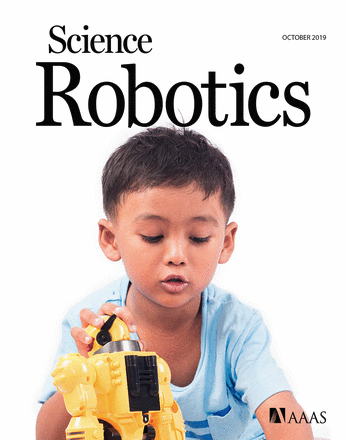
\includegraphics[height=2.2cm]{thumbs/2019-science.png} & Senft, E.,
    \ul{Lemaignan, S.}, Baxter, P., Bartlett, M., Belpaeme, T.
    \newline\href{https://doi.org/10.1126/scirobotics.aat1186}{\textbf{Teaching robots
    social autonomy from in situ human guidance}}
    \newline \textit{Science Robotics} 2019
    & \small A novel human-in-the-loop machine learning approach
    to implement social autonomy in a robot, with several deployments in UK
    public schools. This is a first-in-kind demonstration of learning autonomous
    action policy in a high dimensional, socially complex,
    environment.\textbf{\newline[main study supervisor]} \\


    \vspace{-.20cm}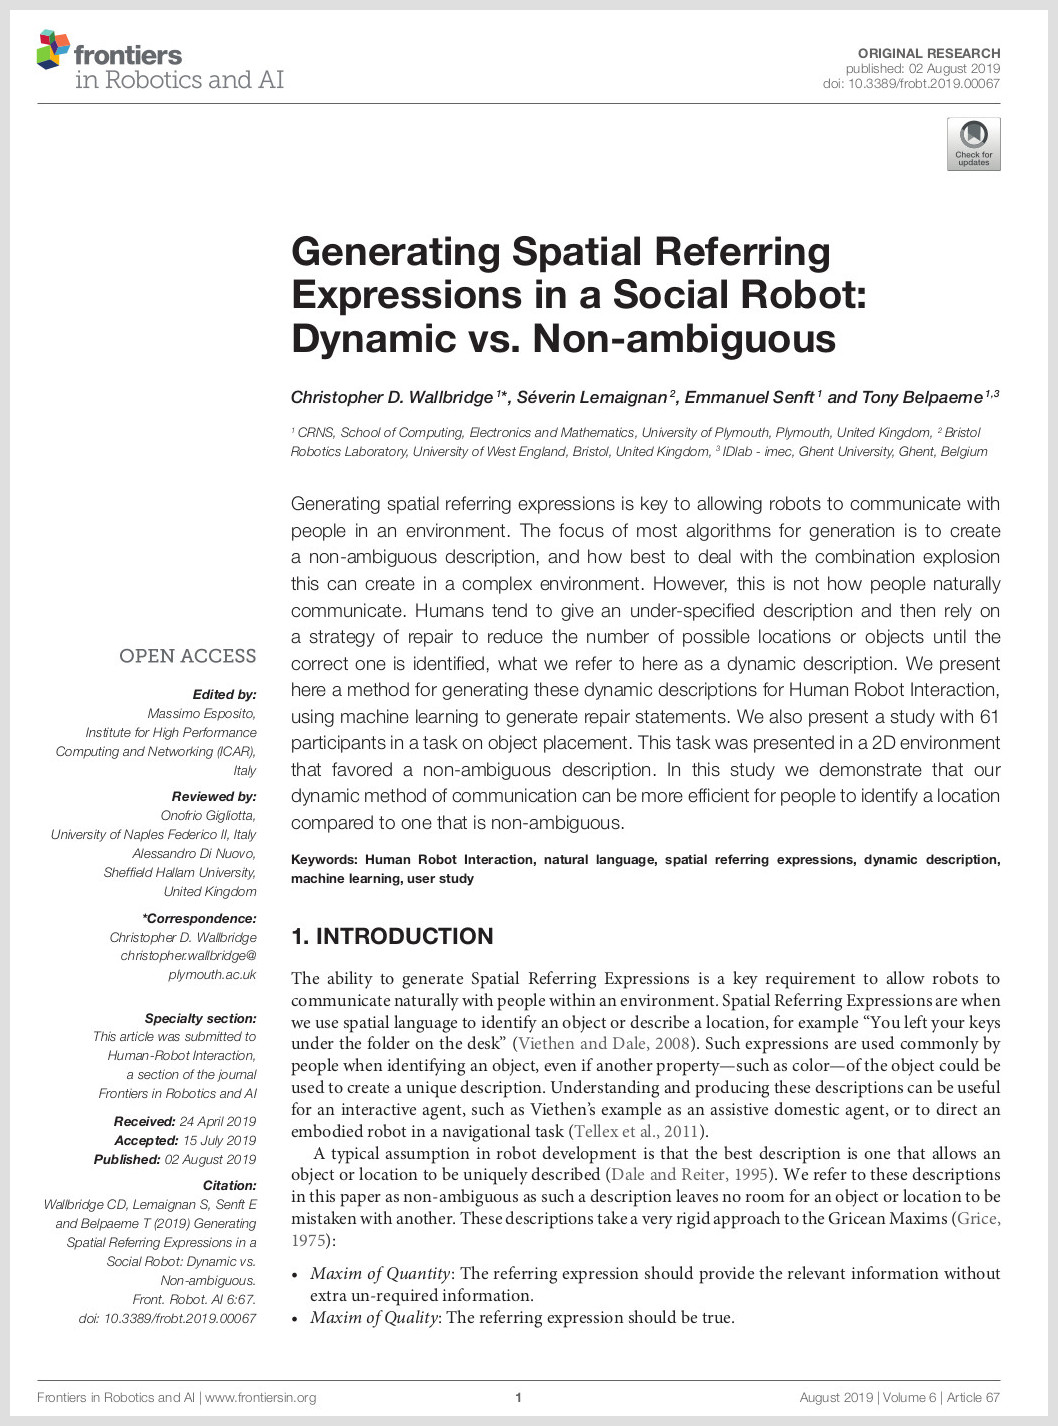
\includegraphics[height=2.2cm]{thumbs/2019-frontiers-chris.jpg} &

    Wallbridge, C., \ul{Lemaignan, S.}, Senft, E., Belpaeme, T.  
    \newline\href{https://doi.org/10.3389/frobt.2019.00067}{\textbf{Generating
    Spatial Referring Expressions in a Social Robot: Dynamic vs Non-Ambiguous}}
    \newline \textit{Frontiers in AI and Robotics} 2019
    & \small Challenges the common understanding that robots should be
    unambiguous: we show that ambiguity is often desirable for fluid and natural
    human-robot interactions.\textbf{\newline[main study supervisor]}  \\

    \vspace{-.20cm}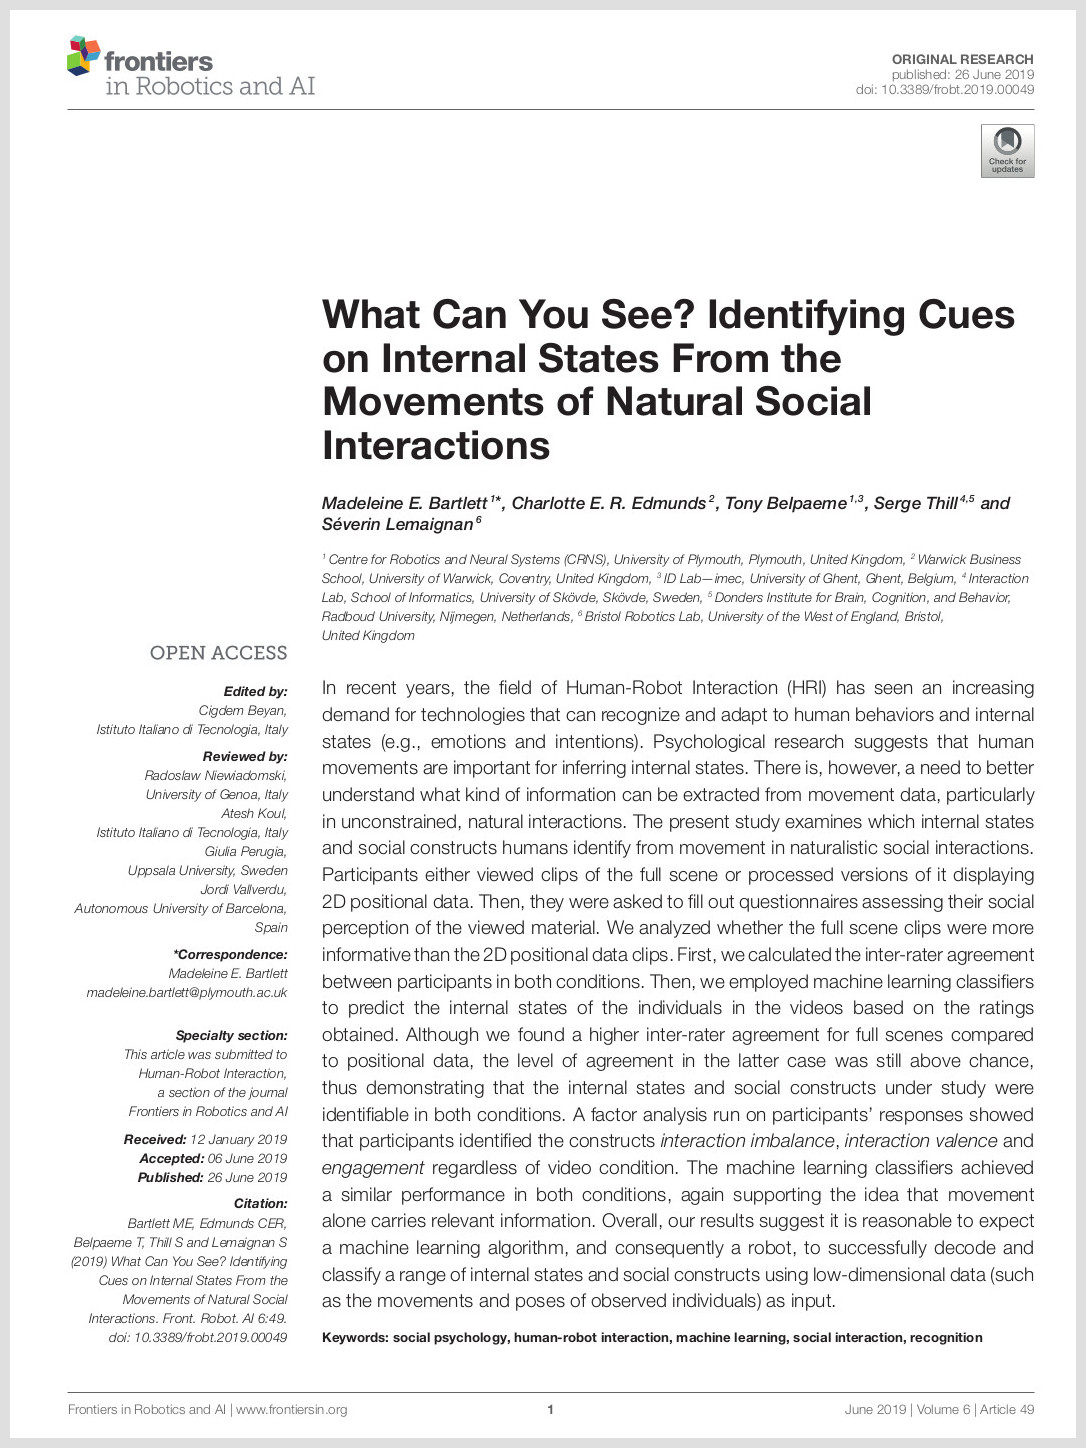
\includegraphics[height=2.2cm]{thumbs/2019-frontiers-maddy.jpg} &

    Bartlett, M., Edmunds, C. E. R., Belpaeme, T., Thill, S., \ul{Lemaignan, S.} 
    \href{https://doi.org/10.3389/frobt.2019.00049}{\textbf{What Can You See? Identifying Cues on Internal States from the
    Kinematics of Natural Social Interactions}} 
    \newline \textit{Frontiers in AI and Robotics} 2019
    & \small Investigates how partially hidden 'internal states' (like emotions,
    cooperativeness, etc) can be decoded from simple visible cues, like
    skeletons. Also demonstrates that social situations can be described along 3
    simple dimensions.\textbf{\newline[main study supervisor]}\\


    \vspace{-.20cm}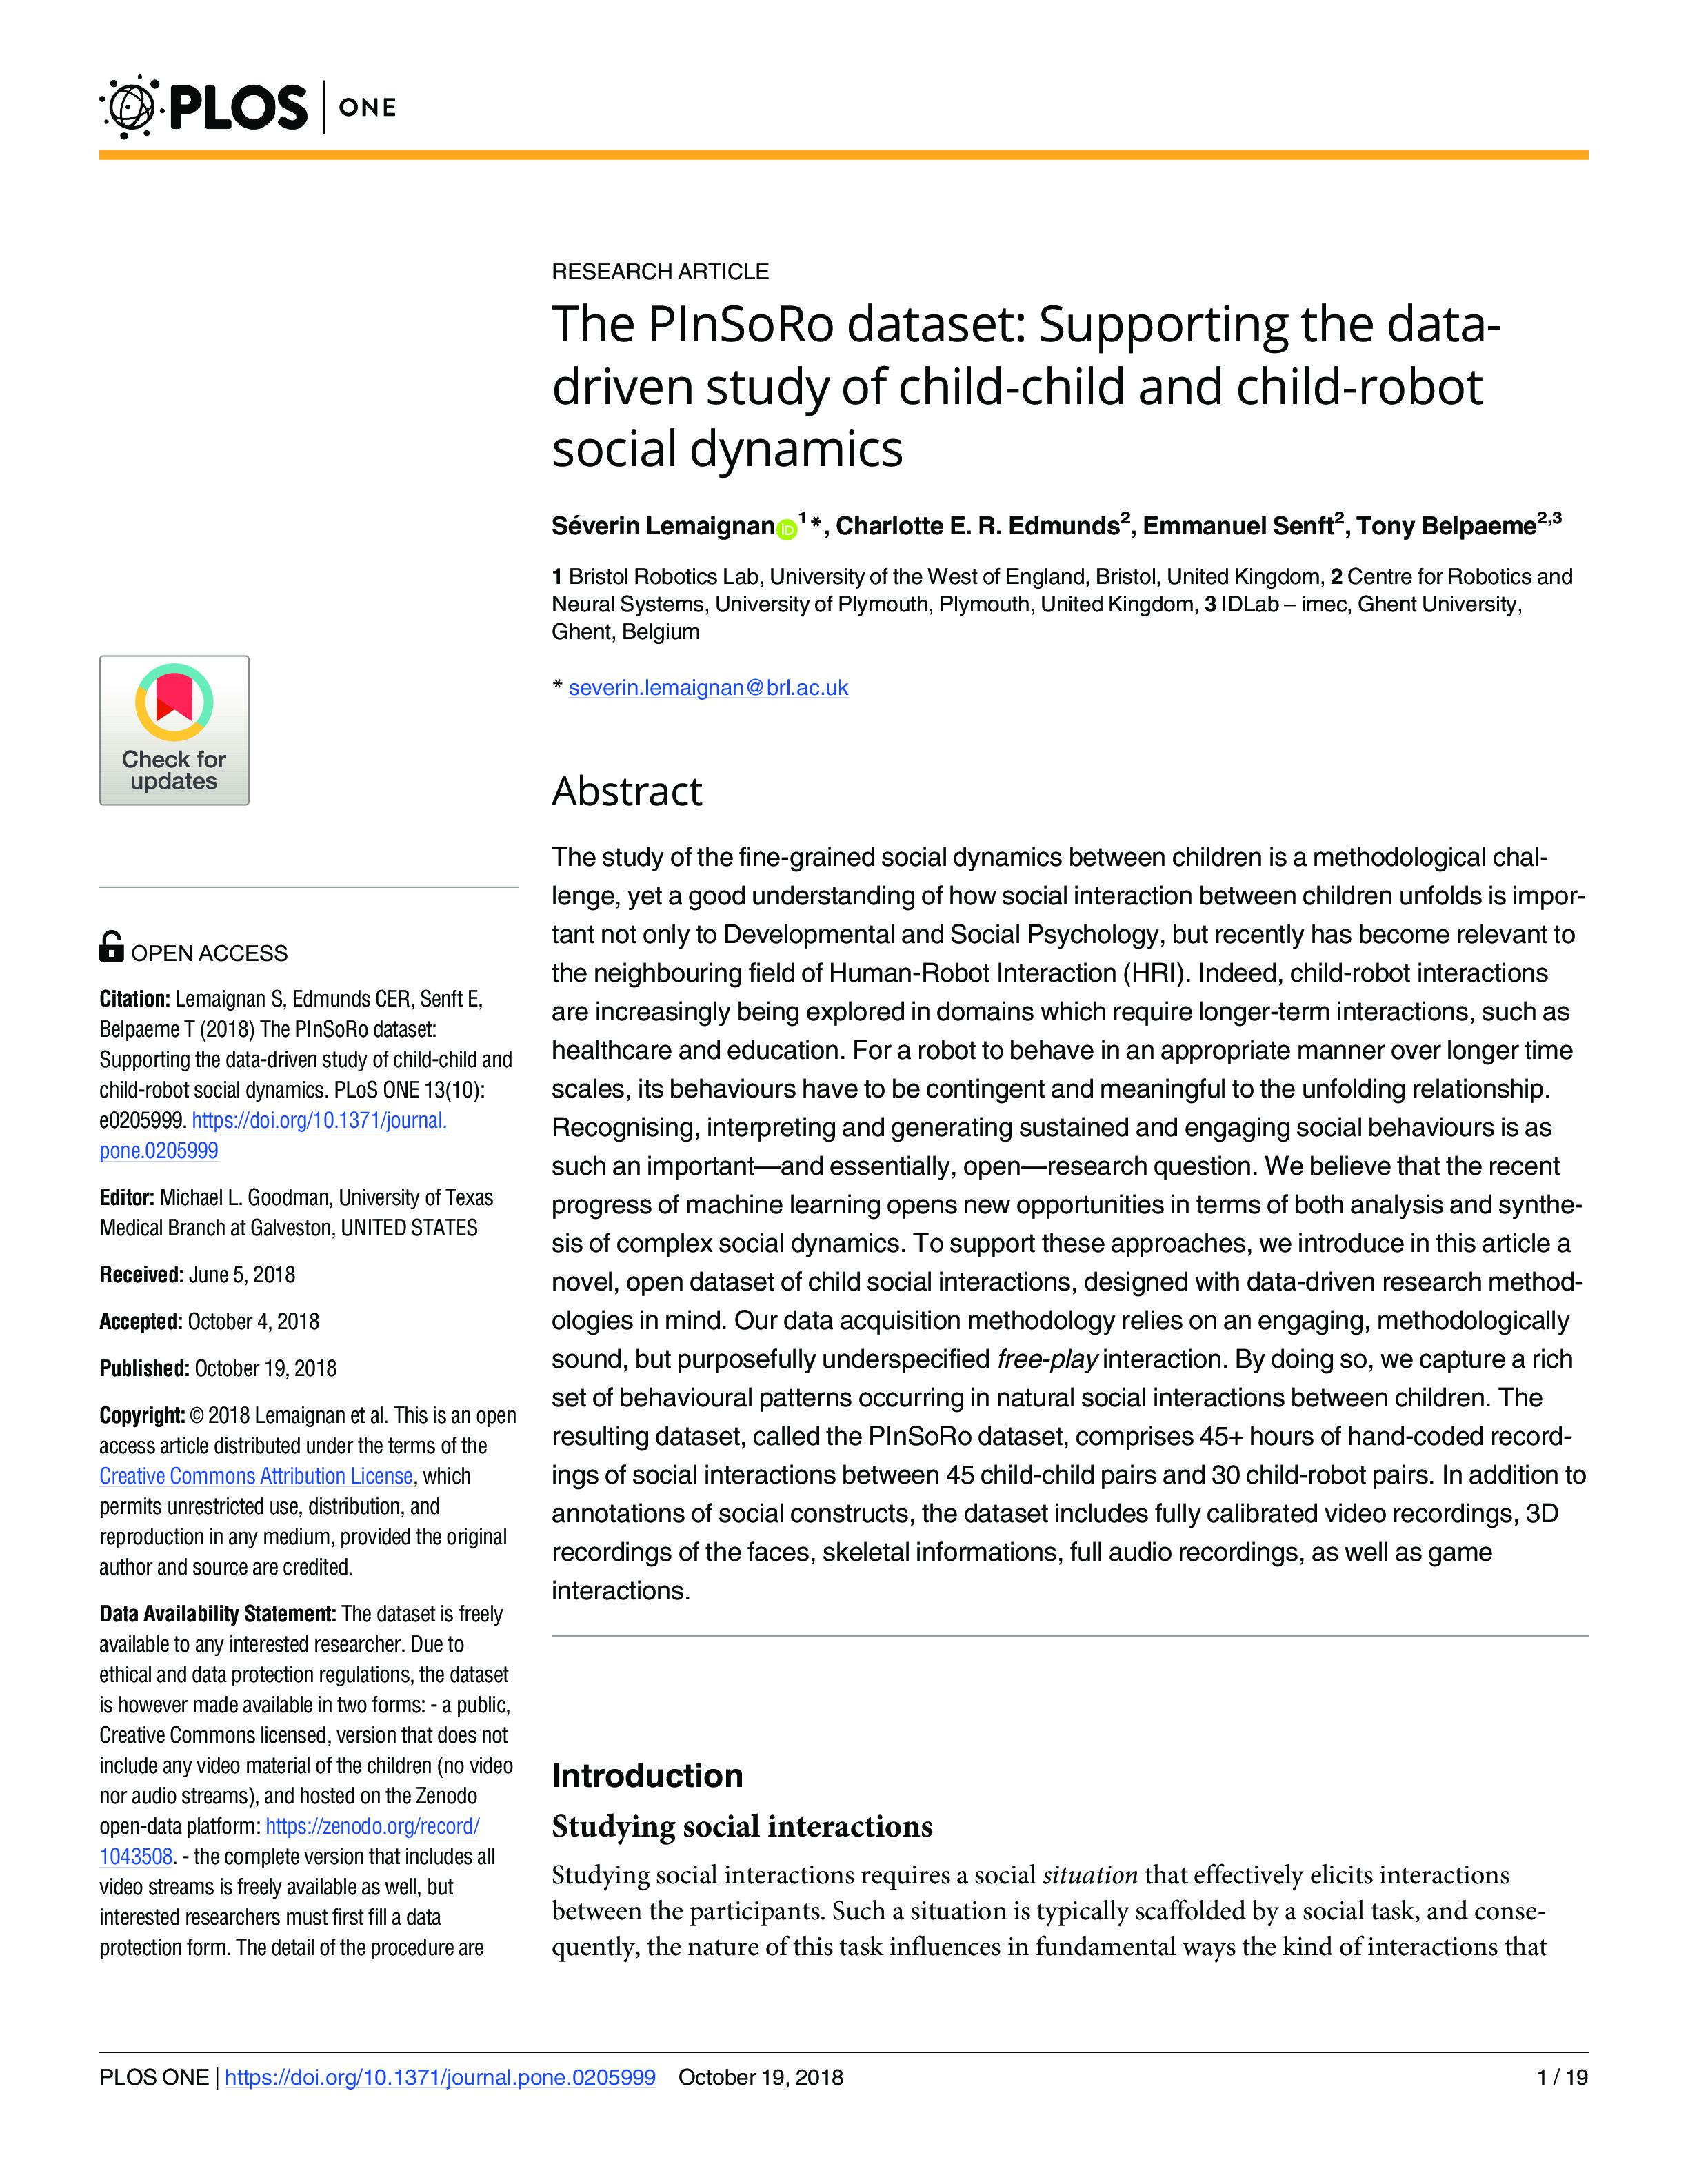
\includegraphics[height=2.2cm]{thumbs/2018-plosone.jpg} &

    \ul{Lemaignan, S.}, Edmunds E. R., C., Senft, E., Belpaeme, T.
    \newline\href{https://doi.org/10.1371/journal.pone.0205999}{\textbf{The
    PInSoRo dataset: Supporting the data-driven study of child-robot social
    dynamics}}
    \newline \textit{PLOS ONE} 2018
    & \small A first-in-kind, large scale dataset of child-child and child-robot social interactions. Design
    with machine learning in mind, this dataset effectively opens up the field
    of data-driven social psychology, with direct applications in AI and social
    robotics.\textbf{[principal investigator]}\\


    \vspace{-.20cm}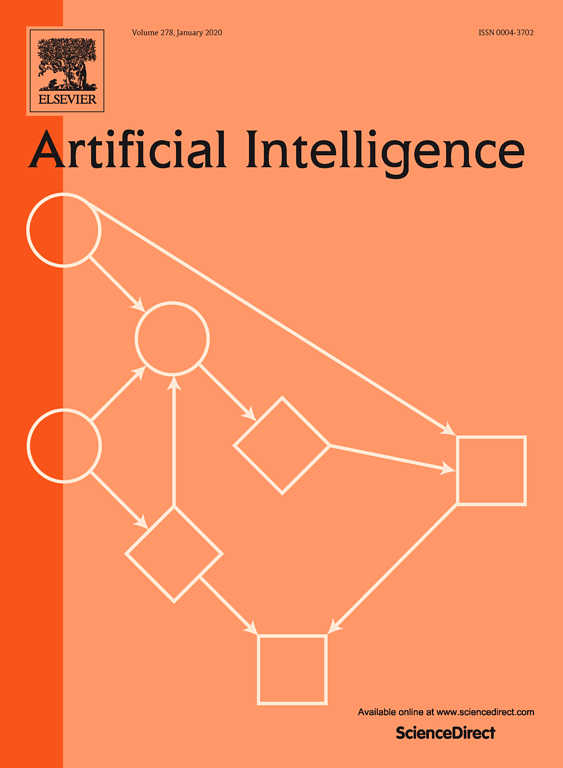
\includegraphics[height=2.2cm]{thumbs/2017-ai-cover.jpg} &

    \ul{Lemaignan, S.}, Warnier, M., Sisbot, E.A., Clodic, A., Alami, R.
    \newline
    \href{https://doi.org/10.1016/j.artint.2016.07.002}{\textbf{Artificial
    Cognition for Social Human-Robot Interaction: An Implementation}}
    \newline \textit{Artificial Intelligence} 2017
    & \small Landmark article: one of the first complete, semantic-aware, robotic architecture for
    human-robot interaction, including symbolic knowledge representation,
    situation assessment, natural language grounding, task planning, human-aware
    motion planning and execution. \textbf{\newline[principal investigator and
    coordinator; 400+ citations]}\\


    \vspace{-.20cm}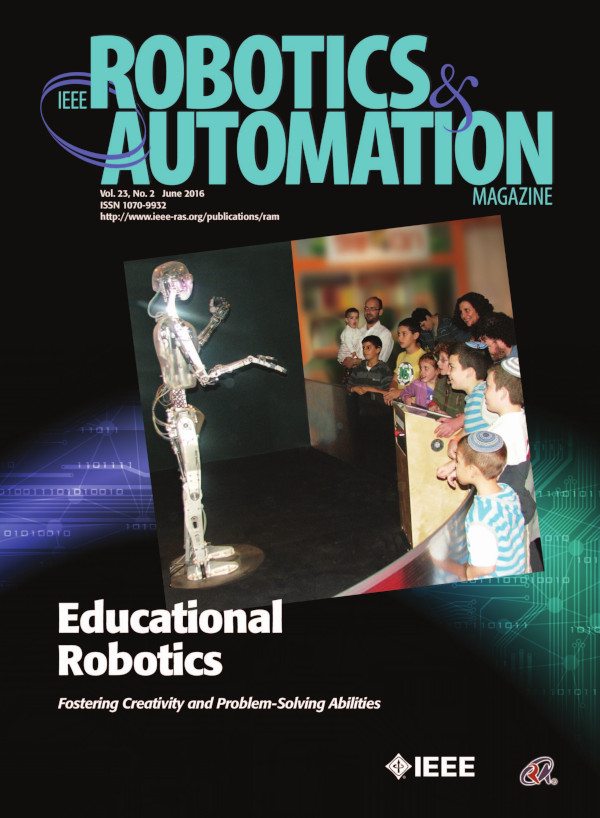
\includegraphics[height=2.2cm]{thumbs/2016-cowriter.jpg} &

    \ul{Lemaignan, S.}, Jacq, A., Hood, D., Garcia, F., Paiva, A., Dillenbourg, P.
    \newline
    \href{https://doi.org/10.1109/MRA.2016.2546700}{\textbf{Learning by
    Teaching a Robot: The Case of Handwriting}}
    \newline \textit{Robotics and Automation Magazine} 2016
    & \small Long-term studies with children and
    therapists, where we \emph{reverse} the social role of the
    robot to significantly improve the children' self-confidence. A landmark in
    social robotics for education. \textbf{\newline[principal investigator; 300+
    citations} \textbf{]}\\


    \vspace{-.20cm}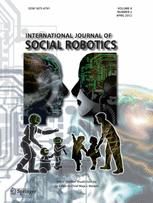
\includegraphics[height=2.2cm]{thumbs/2012-grounding.jpg} &

    \ul{Lemaignan, S.}, Ros, R., Sisbot, E. A., Alami, R., Beetz M.
    \href{https://doi.org/10.1007/s12369-011-0123-x}{\textbf{Grounding
    the Interaction: Anchoring Situated Discourse in Everyday Human-Robot
    Interaction}} 
    \newline \textit{Intl Journal of Social Robotics} 2012

    & \small In this paper, I show how symbolic knowledge representation can be
    used by robot to ground natural language interactions, also taking into
    account the unique perspective of the human interactor.
    \textbf{\newline[principal investigator; 100+ citations]}\\

    \vspace{-.20cm}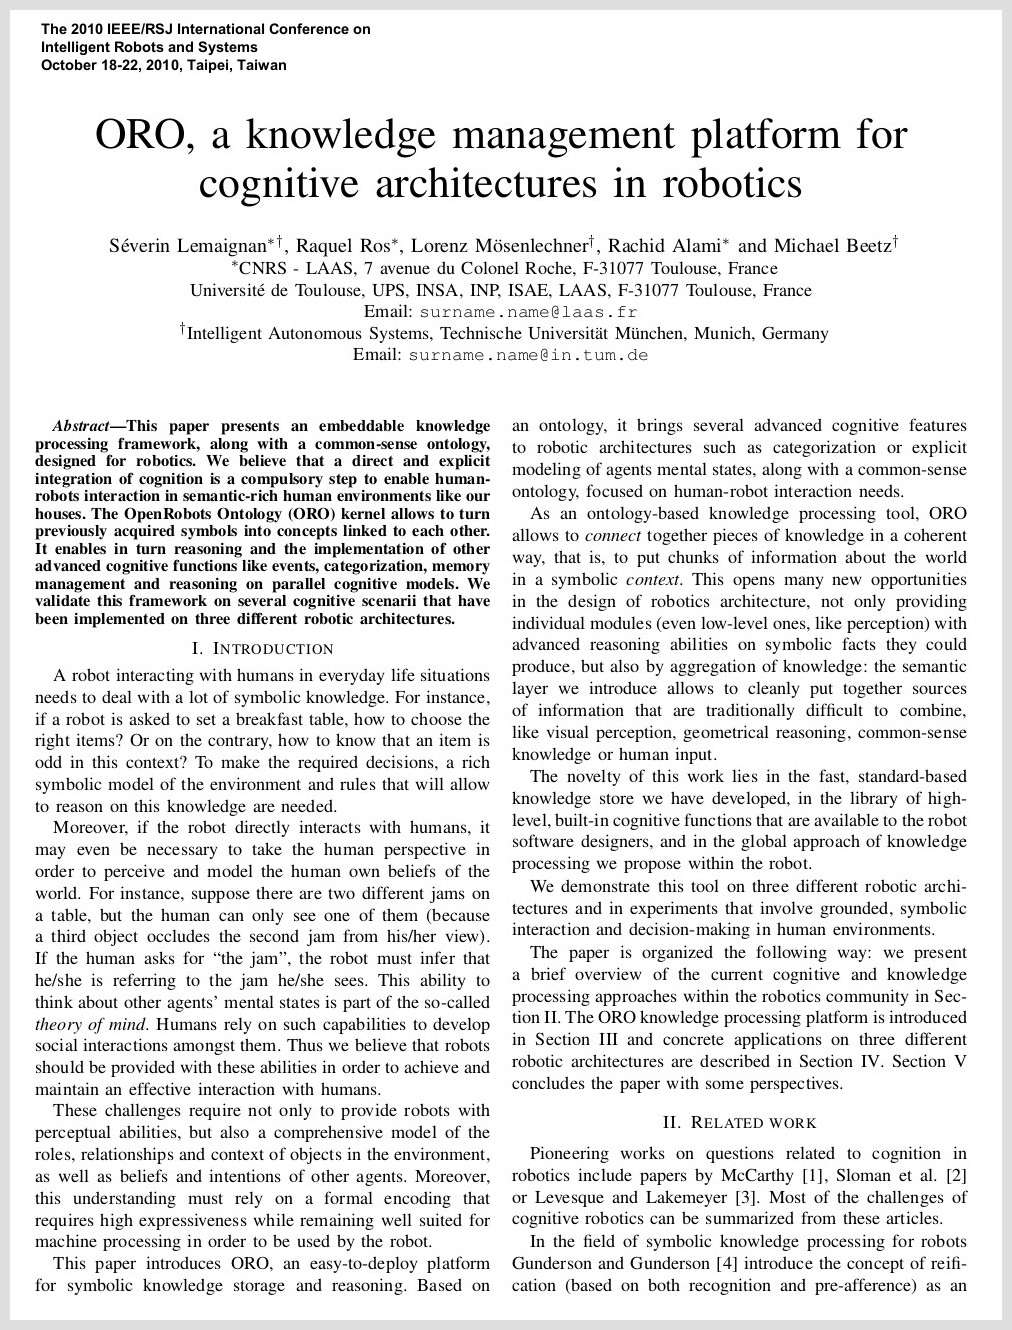
\includegraphics[height=2.2cm]{thumbs/2010-oro.jpg} &
    \ul{Lemaignan, S.}, Ros, R., Mösenlechner, L., Alami, R., Beetz, M.
    \newline\href{https://doi.org/10.1109/IROS.2010.5649547}{\textbf{ORO, a Knowledge Management Module for Cognitive Architectures in
    Robotics}}
    \newline \textit{IEEE IROS} 2010

    & \small One of the very first knowledge base designed and
    integrated in service robots. Pioneering work which played a key role in
    understanding how intelligent robot can represent their
    knowledge to facilitate communication with humans.
    \textbf{\newline[principal investigator; 200+ citations]}\\

\end{tabular}
%}



\subsection{Peer recognition}


\subsubsection{Significant International Editorial roles}

\begin{tabular}{p{0.15\linewidth}p{0.8\linewidth}}
    {\bf 2025} & {General Chair of the IEEE/ACM HRI'25 conference} \\
    {\bf 2018--} & {Associate Editor, Frontiers in Robotics and AI} \\
    {\bf 2018--} & {Program Committee of major international conferences in AI and
    robotics: IROS'16--'18; IJCAI'17--'21; HRI'16--'24; HAI'18; AAMAS'19;
    RSS'20} \\
    {\bf 2017--} & {Organisation committee of the IEEE/ACM HRI conference, '17--'24} \\
    {\bf 2019} & {UK TAROS conference on Autonomous Robotis Systems}{co-coordinator} \\
\end{tabular}

%	{\bf 2016}{Program Chair, Workshop on Cognitive Architectures for Social HRI}{HRI 2016} {} {} {} 
%	{\bf 2013}{Steering Committee, Intl. Workshop on MORSE for HRI}{HRI 2014} {} {} {} 
%	{\bf 2013}{Program Committee, Workshop on Developmental Social Robotics}{IROS 2013} {} {} {} 
%	{\bf 2012}{Steering Committee, Intl. Workshop on MORSE and its Applications}\\ 
%	{\bf 2008--2009}{Steering Committee, Cognitive Sciences' Young Researchers Conference 2009}\\

\subsubsection{Awards and Honours}

\begin{tabular}{p{0.15\linewidth}p{0.8\linewidth}}
    {\bf HRI'2017} & {Best Paper Award 'Design'} \\
    {\bf HRI'2016} & {Best Paper Award 'Methods and Theory'} \\
    {\bf AAAI'2015} & {Best Video Award in Artificial Intelligence} \\
    {\bf AAAI'2014} & {Best Late Breaking Report Award} \\
    {\bf 2012} & {\underline{\textbf{Best PhD in Robotics}}, CNRS} \\
    {\bf 2012} & {\underline{\textbf{PhD with High Distinction}} (``Summa Cum
	Laude''), TU Munich} \\
    {\bf Ro-Man'2010} & {Best Paper Award} \\
%\cvlistitem{\textbf{Gold Medal} (top ten students), ENSAM ParisTech 2006}
\end{tabular}

\subsubsection{Recent International Keynotes and Invited Talks}

\begin{itemize}
    \item {\textbf{End-to-end Participatory Design} -- \textit{keynote}, 2023,
        NAVERLab HRI Symposium, Grenoble} 
    \item {\textbf{Cognitive Architectures for Social Robots} --
        \textit{keynote}, 2023, HRI Symposium, Tel-Aviv} 
    \item {\textbf{ROS4HRI} -- \textit{keynote}, 2022, ROSCon'22, Kyoto} 
    \item {\textbf{Robots for Learning} -- \textit{invited speaker}, 2019, Robot4SEN,
Vocational Training Council, Kong Kong} 
\item {\textbf{From Big Data to Social Robotics} -- \textit{keynote}, 2019, UK
    RAS conference, Loughborough, UK} 
\item {\textbf{Theory of Mind and Joint-action} -- \textit{keynote}, 2018, Robotics Science and System, Pittsburgh, USA} 
\item {\textbf{Robots for Learning} -- \textit{keynote}, 2018, Symposium on Robots for Language Learning,  Koç University, Istanbul, Turkey} 
\end{itemize}


\subsubsection{Recent International expert \& advisory roles}

\begin{tabular}{p{0.15\linewidth}p{0.8\linewidth}}
    {\bf 2023} & {\bf Invited to co-author the upcoming \emph{Responsible
    Robotics} roadmap; Dagsthul seminar}  \\
    {\bf 2020--2024} & {\bf Invited member of the International HRI Steering Committee} \\
    {\bf 2021--} & {Expert on Ethics of Child-Robot Interaction; EU JRC/UNICEF} \\
    {\bf 2017--} & {EU H2020 member on the Peer Review College} \\
    {\bf 2019--} & {Full member of the UK EPSRC College} \\
    {\bf 2019--} & {Invited PhD committee examiner, 6 times since 2019, in Sweden
(Örebro, Uppsala, KTH), Germany (Bielefeld), France (LAAS-CNRS), UK (Bristol
Robotics Lab)} \\
    {\bf 2019} & {Invited Expert in Child-Robot Interaction, robot4SEN project,
	VTC, Hong Kong} \\
    {\bf 2018--} & {Senior Scientific Adviser for South-West UK SMEs} {EU H2020 SABRE project} \\
\end{tabular}

\subsubsection{Recent Contributions to Policy making}

\begin{tabular}{p{0.15\linewidth}p{0.8\linewidth}}
    {\bf 2020 --} & {Expert Collaborator for the European Joint Research
Centre, contributing to the UNICEF Guidelines for Responsible Child-Robots
Interactions} \\
    {\bf 2019} & {Invited panel by the EU Research Executive Agency, MSCA AI
Cluster, sharing expertise in Human-Robot Interaction} \\
    {\bf 2018--2020} & {BRL strategic planning}{involved in discussion about
Intelligent Manufacturing; HRI systems; Assistive robotics with key UK policy
makers, incl. BEIS Secretary of State Greg Clark} \\
\end{tabular}



\section{Additional Information}

\subsection{Career breaks, diverse career paths and major life events}

\eu{You may include a short factual explanation of career breaks or diverse career paths such as secondments, volunteering, part-time work, time spent in different sectors or the effects of major life events such as long term illness as well as the effects of pandemic restrictions on research productivity.}

\subsection{Other contributions to the research community}

\eu{You may include a list of particularly noteworthy contributions to the research community you have made other than research achievements and peer recognition and a short explanation of these contributions. The purpose of this section is to allow the panels to take a more rounded view of your career and achievements and to ensure that any additional responsibilities, commitments and leadership roles that you have taken on beyond your individual research activities are recognised and taken into account.}

\TODO{say smthg about leadership position at BRL + PAL}
%%%%%%%%%%%%%%%%%%%%%%%%%%%%%%%%%%%%%%%%%%%%%%%%%%%%%%%%%%%%%%%%%%%%%%%%%%%%%
%%%%%%%%%%%%%%%%%%%%%%%%%%%%%%%%%%%%%%%%%%%%%%%%%%%%%%%%%%%%%%%%%%%%%%%%%%%%%
%%%%%%%%%%%%%%%%%%%%%%%%%%%%%%%%%%%%%%%%%%%%%%%%%%%%%%%%%%%%%%%%%%%%%%%%%%%%%

%I \textbf{contributed significantly to the framing
%of the emerging field of data-driven HRI}, also releasing of the PInSoRo open
%dataset (\href{https://doi.org/10.5281/zenodo.1043507}{10.5281/zenodo.1043507}),
%a \textbf{one-in-a-kind dataset of child-child and child-robot social
%interactions}.
%


%\subsection{Host institution}\label{host-institution}}
%
%The \emph{Bristol Robotics Laboratory (BRL)} is the largest co-located
%and most comprehensive advanced robotics research establishment in the
%UK. It is a joint venture between the University of the West of England
%and the University of Bristol. BRL's multidisciplinary approach aims to
%create autonomous devices capable of working independently, with each
%other, or with humans. BRL draws on robotics, electrical \& mechanical
%engineering, computer science, psychology, cognitive science and
%sociology. BRL has an international reputation as a leading research
%centre in advanced robotics research and has over 250 researchers
%working on a broad portfolio of topics: HRI, collective robotics, aerial
%robotics, neuro-inspired control, haptics, control systems, energy
%harvesting and self-sustaining systems, rehabilitation robotics, soft
%robotics and biomedical systems. BRL has many collaboration
%partnerships, both national and international, and is experienced in
%managing large multi-site projects. BRL has support from two embedded
%units specialising in business and enterprise, together with an
%incubator and successful track record of spin-outs.





